\documentclass{article}
\usepackage[utf8]{inputenc}
\usepackage{amsmath, amssymb, bm}
\usepackage{gensymb}
\usepackage{graphicx}

\begin{document}
	\textbf{Trig Inequality 2:} For all angles $\theta < 0$,
	$$\theta < \sin{(\theta)}$$
	\textbf{Proof:}
	Let $\theta < 0$ be an arbitrary real angle. \\\\
	Case 1: Suppose $\theta \leq -\frac{\pi}{2}$. Since the range of sine is $[-1, 1]$, then
	$$-1 \leq \sin{(\theta)}$$
	Since $-\frac{\pi}{2} \approx -1.571 < -1$, then
	\begin{align*}
		\theta \leq -\frac{\pi}{2} < \sin{(\theta)}
	\end{align*}
	which is what we wanted to show. \\\\
	Case 2: Suppose $-\frac{\pi}{2} < \theta < 0$. Then the terminal side of the angle $\theta$ lies in Quadrant IV and can be represented by Figure 1 below.
	\begin{figure}[h!]
		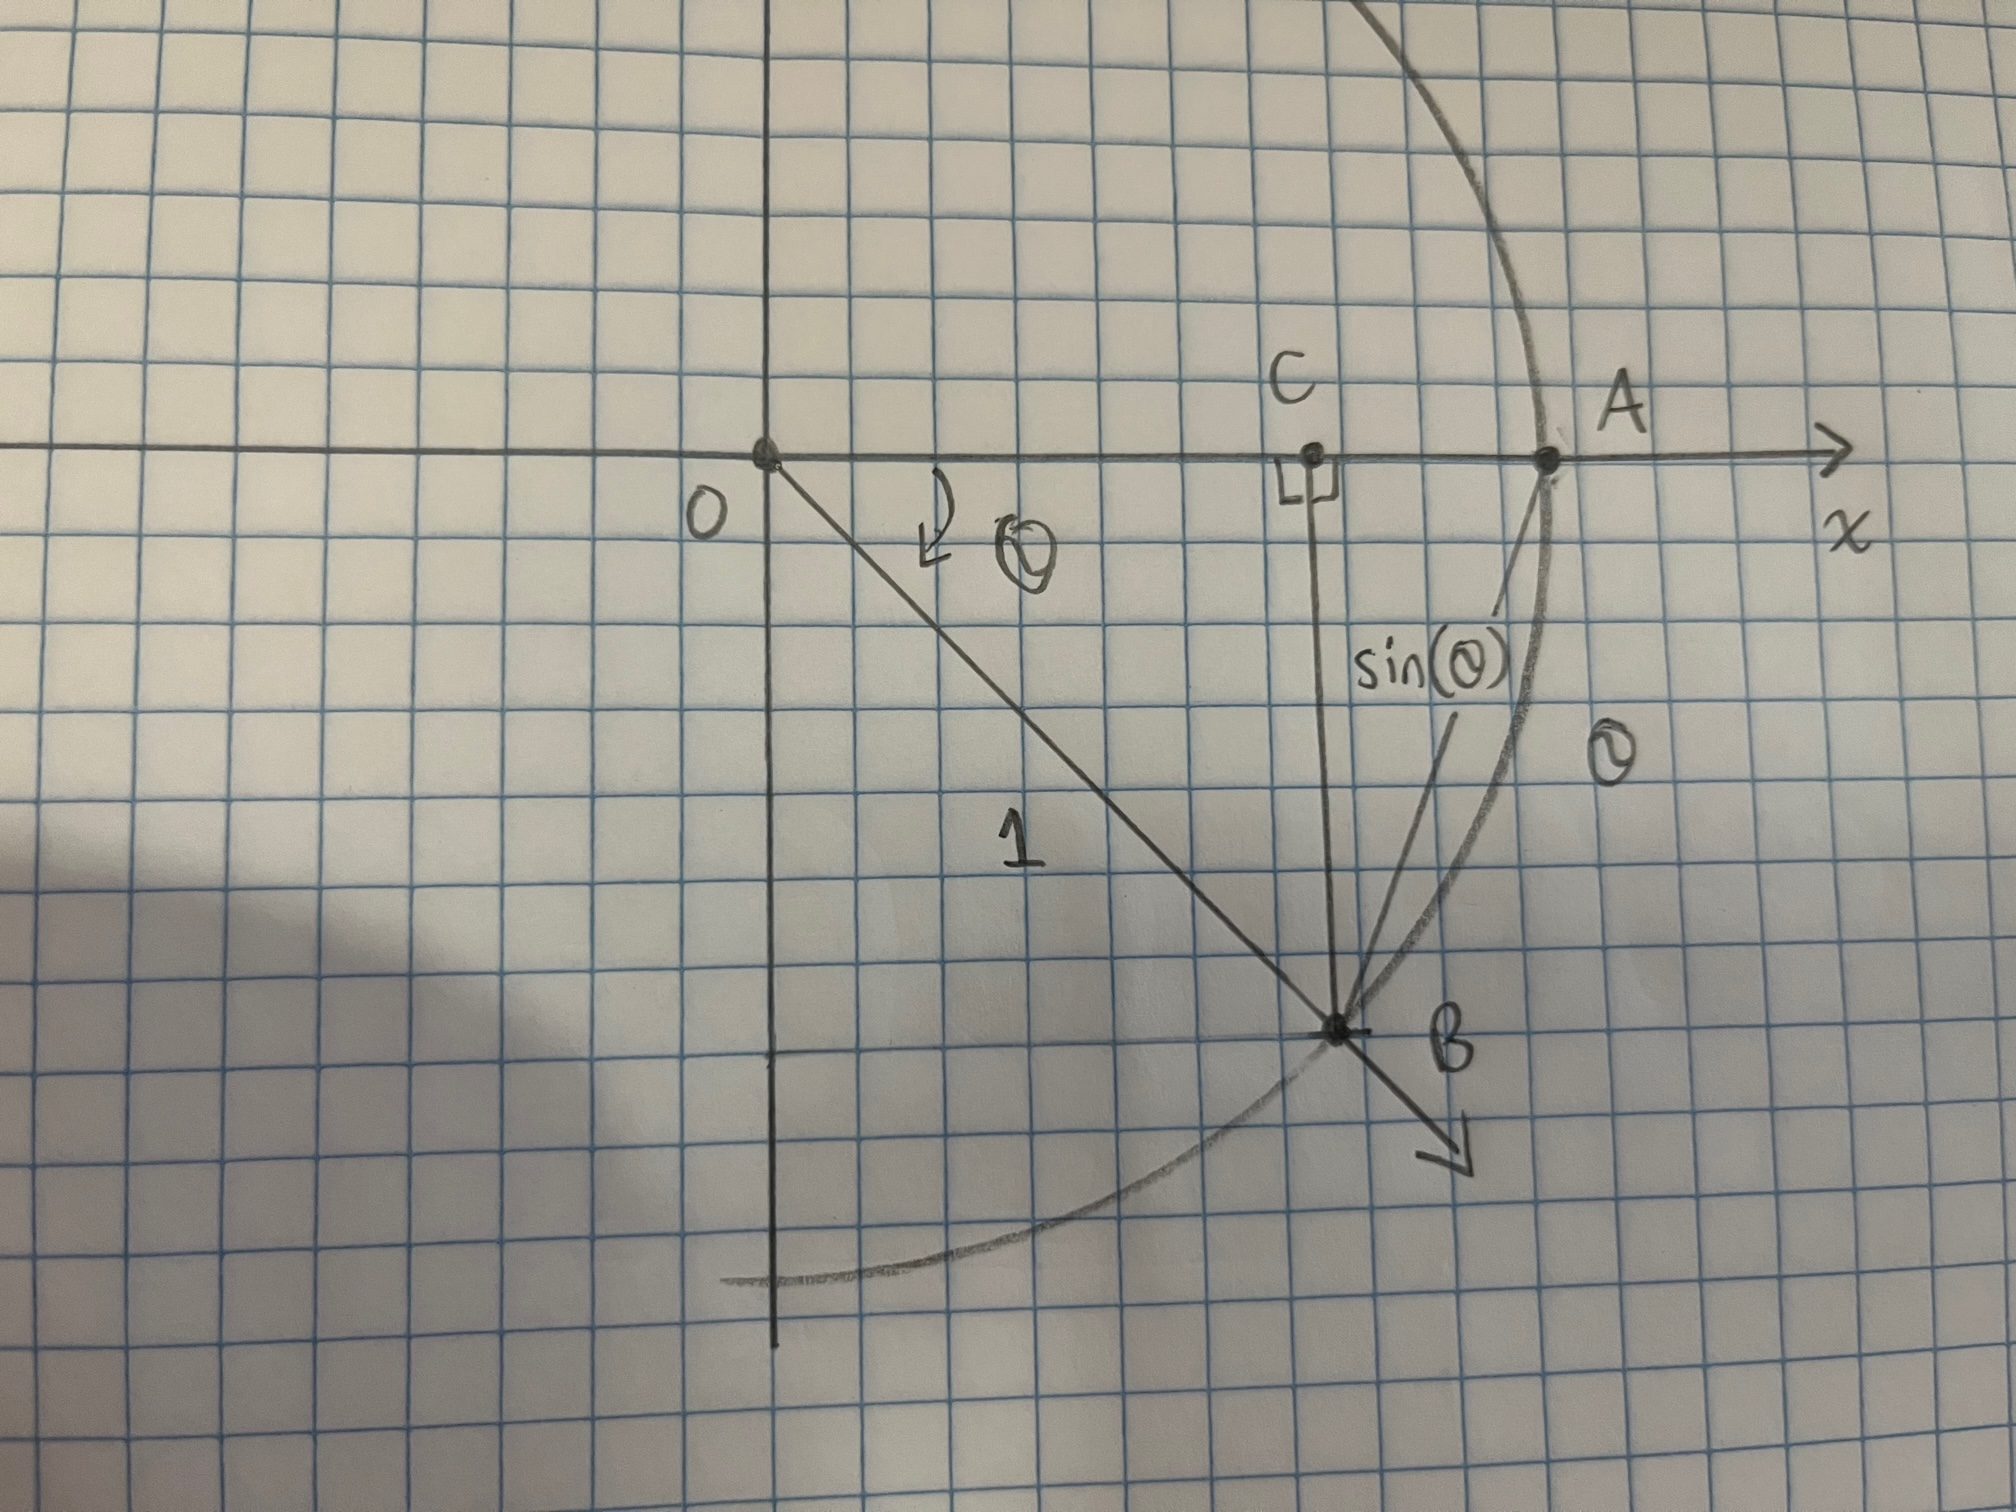
\includegraphics[width=\linewidth]{Trig_Figure_2.jpg}
		\caption{Angle lies in QIV}
	\end{figure} \\
	By definition, $\sin{(\theta)} = -|BC|$. By the definition of radian measure, the length of arc $AB = \theta$.  \\\\
	Since $\triangle ABC$ is a right triangle, the Pythagorean Theorem applies to it. So, since $|CA| > 0$, then
	\begin{align*}
		|CA|^2 &> 0 \\
		|CA|^2 + |BC|^2 &> |BC|^2 \\
		|AB|^2 &> |BC|^2 \tag{Pythag. Thrm.} \\
		|AB| &> |BC| \tag{Length is positive} \\
		-|AB| &< -|BC| \\
		-|AB| &< \sin{(\theta)}
	\end{align*}
	From looking at the figure, it is geometrically intuitive \footnote{This is all we can say without having access to a more precise definition of arc length.} that the arc $AB$ is a longer length than the line segment $AB$. Since $\text{arc }AB$ is an oriented arc, and the angle $\theta$ rotates clockwise, then $\text{arc }AB < 0$, so being ``longer'' means its numerical value is less than $-|AB|$.
	\begin{align*}
		\text{arc }AB &< -|AB| < \sin{(\theta)} \\
		\theta &< -|AB| < \sin{(\theta)}
	\end{align*}
	
	The inequality holds in both cases, thus for all $\theta < 0$,
	$$\theta < \sin{(\theta)}$$
\end{document}